\section{Coordinate descent deconvolution}\label{cd}
Coordinate descent methods are a family of algorithms. Various variants exist\cite{richtarik2016distributed, richtarik2016parallel}, but they share one common idea: Most of our problems become simple when we reduce the number of dimensions. Deconvolving a whole image is difficult. But deconvolving a single pixel is easy. As we will show in section \ref{cd:deriving}, we can derive a closed form solution\footnote{Deriving a formula which we can implement in a few lines of code.} for deconvolving a single pixel. We then iterate over all pixels, possibly several times, until we converge to a deconvolved image. 

This is the idea behind coordinate descent methods. By reducing the dimensions of the problem, we can often find an optimization algorithm where each iteration is "cheap" to compute. In these cases, coordinate descent methods produce competitive results\cite{nesterov2012efficiency, nesterov2013gradient}.

For a deconvolution algorithm in radio astronomy, we need three parts: An optimization algorithm, a regularization, and an optimization objective. We use coordinate Descent as the optimization algorithm, take Elastic Net as the regularization and use the following objective function:

\begin{equation}\label{cd:deconv}
\underset{x}{minimize} \: \frac{1}{2} \left \| I_{dirty} - x * PSF \right \|_2^2 + \lambda ElasticNet(x)
\end{equation}

As we have shown before, the objective function consists of two parts. The data term $\left \| I_{dirty} - x * PSF \right \|_2^2$ and the regularization term $ElasticNet(x)$. The data term forces the image to be as close to the measurements as possible which forces the image to be as close to the measurements as possible, the regularization term forces the image to be as consistent as possible with our prior knowledge. The parameter $\lambda$ is a weight that either forces more or less regularization. It is left to the user to define for each image. We will derive the coordinate descent algorithm that optimizes the objective \eqref{cd:deconv} in section \ref{cd:deriving}. First, let us explain what the elastic net regularization does.

\subsection{Elastic net regularization} \label{cd:reg}
\begin{figure}[h]
	\centering
	\begin{subfigure}[b]{0.3\linewidth}
		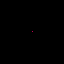
\includegraphics[width=\linewidth]{./chapters/03.distribution/L1.png}
		\caption{Effect of the pure L1 norm ($\lambda$ = 1.0) on a single point source.}
		\label{cd:elastic:L1}
	\end{subfigure}
	\begin{subfigure}[b]{0.3\linewidth}
		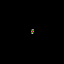
\includegraphics[width=\linewidth]{./chapters/03.distribution/L2.png}
		\caption{Effect of the pure L2 norm ($\lambda$ = 1.0) on a single point source.}
		\label{cd:elastic:L2}
	\end{subfigure}
	
	\caption{Effect of the L1 and L2 Norm separately.}
	\label{cd:elastic}
\end{figure}


This regularization is a mixture between the L1 and L2 regularization. The Figure \ref{cd:elastic} shows the effect of the L1 and L2 norm on a single star. The L1 regularization forces the image to contain few non-zero pixels as possible. It encodes our prior knowledge that the image will contain stars. The L2 regularization on the other hand "spreads" the single star across multiple pixels. This forces the image to represent extended emissions, like hydrogen cloud, with a large number of non-zero pixels (the L1 norm tends to break extended emissions apart, only using a handful of non-zero pixels). The L2 norm was already used in other image reconstruction algorithms in radio astronomy\cite{ferrari2014distributed}, with the downside that the resulting image will not be sparse.

Elastic net mixes these two norms together, becoming "sparsifying L2 norm". It retains the sparsifying property of the L1 norm, while also keeping extended emissions in the image. Formally, elastic net regularization is defined as the following:

\begin{equation}\label{cd:elastic:formula}
ElasticNet(x) = \: \alpha \left \|x \right \|_1 + \frac{1-\alpha}{2}  \left \|x \right \|_2
\end{equation}

Elastic net has three properties which make it an interesting regularization for coordinate descent: It was shown to speed up convergence rates compared to the pure L1 or L2 norm\cite{friedman2010regularization}, is a separable function, and has a closed form solution. The first property was not further investigated in this work. The second property, separability, means that we can calculate the regularization for each pixel independently of each other, and we still arrive at the same result. Lastly, we can find a simple formula for each pixel that applies the elastic net regularization:

\begin{equation}\label{cd:elastic:closed}
\lambda ElasticNet(pixel) = \: \frac{max(pixel - \lambda * \alpha, 0)}{1+\lambda(1 - \alpha)}
\end{equation}

The closed form solution \eqref{cd:elastic:closed} of the elastic net regularization is also a mixture of the closed form solutions of the L1 and L2 norm. The closed form solution of the L1 norm is shrinkage: $max(pixel - \lambda, 0)$, we reduce the pixel value by $\lambda$ and clamp negative values. For the L2 norm, we divide the pixel value: $\frac{pixel}{1+\lambda}$.

%Proximal operator But the second property leads to an optimization algorithm 

Note that the shrink operation in this project always clamps negative pixels to zero. We constrain the image to only contain zero or positive pixel values. This has become a widely used constraint in radio interferometric image reconstruction and may lead to improved image quality\cite{mcewen2011compressed}.

Elastic net is the regularization we use throughout this work. It is separable (we can calculate it for each pixel independently) and has an easy to compute closed form solution.


\subsection{Deriving the basic coordinate descent deconvolution algorithm}\label{cd:deriving}
In this section we derive the basic coordinate descent deconvolution algorithm, which minimizes the objective \eqref{cd:deconv}. Coordinate descent methods have a tendency to need a more iterations to converge compared to other methods like gradient descent. However, when a single iteration is cheap to compute, they can be faster in practice\cite{shalev2011stochastic}. The elastic net regularization has an easy to compute closed form solution \eqref{cd:elastic:closed}, and a single iteration is cheap to compute.

We call the coordinate descent algorithm described here "basic". Other coordinate descent algorithms in the literature\cite{richtarik2016parallel,fercoq2015accelerated, richtarik2016distributed} can be seen as generalizations of the "basic" algorithm. The basic algorithm optimizes a single pixel at each iteration, while other algorithms can optimize one or several pixels. 
%We look at the basic coordinate descent algorithm first and use it as a baseline for comparing different coordinate descent algorithms.

In this section, we derive the basic coordinate descent algorithm that optimizes a single pixel in each iteration, and iterates over all pixels several times, with a specific strategy, until convergence. There are three types of iteration strategy we can choose:
\begin{enumerate}
	\item Random: where we choose a pixel to optimize uniformly at random.
	\item Greedy: where we first choose the pixel which minimizes our objective the most
	\item Cyclic: where we choose a subset of pixels and cycle through them until convergence. 
\end{enumerate}

The iteration strategy is not important for convergence. We can for example create a mixture of the different strategies and the algorithm would still converge to the optimum. However, the strategy we choose has an impact on how many iterations we need until convergence. For example: if the image consists of a single star in the center of the image, a greedy strategy would first optimize the pixel at the center, while a random strategy may waste the computing resources in checking every other pixel several times before finally landing on the center. In this implementation, we chose the greedy strategy. Each iteration takes the best possible step towards the optimum. We arrive at the following coordinate descent algorithm in pseudocode:


\begin{lstlisting}
dirty = IFFT(Gridding(visibilities))
residuals = dirty

x = new Array
objectiveValue = SUM(residuals * residuals) + P(x)
oldObjectiveValue = objectiveValue

do 
{
	oldObjectiveValue = objectiveValue

	//the core of the algorithm
	pixelLocation = GreedyStrategy(residuals)
	oldValue = x[pixelLocation]
	optimalValue = oldValue + Minimize(residuals, psf, pixelLocation)
	optimalValue = ApplyElasticNet(optimalValue, lambda, alpha)
	
	//housekeeping
	x[pixelLocation] = optimalValue
	residuals = (dirty - Convolve(x, psf))
	objectiveValue = 0.5 * SUM(residuals * residuals) + lambda * ElasticNet(x)
} while (oldObjectiveValue - objectiveValue)  < epsilon
\end{lstlisting}

The core of the algorithm consists of the three functions: $GreedyStrategy()$, $Minimize()$ and $ApplyElasticNet()$. The function $GreedyStrategy()$ will be discussed in Section \ref{cd:efficient}. The function $ApplyElasticNet()$ was already described in equation \eqref{cd:elastic:closed}. The $Minimize()$ function is responsible for minimizing the data term of our objective \eqref{cd:deconv}. Because we only minimize a single pixel, we are dealing with a one dimensional minimization problem and can derive a closed form solution for it.

When we only have one pixel to minimize, the data term of our objective \eqref{cd:deconv} reduces itself to a parabola. We derive the standard parabola form in \eqref{cd:deriving:derivation}, where $\langle x, y\rangle$ is the inner product(element-wise multiplication followed by a sum over all elements):

\begin{equation} \label{cd:deriving:derivation}
\begin{split}
Minimize(pixel) & = \left \| I_{res} - PSF * pixel \right \|_2^2\\
Minimize(pixel) & = (I_{res} - PSF * pixel)^2\\
Minimize(pixel) & = \langle I_{res}, I_{res} \rangle - 2\langle I_{res},PSF\rangle * pixel + \langle PSF, PSF \rangle * pixel^2\\
Minimize(pixel) & = \langle PSF, PSF \rangle * pixel^2 - 2\langle I_{res},PSF\rangle * pixel + \langle I_{res}, I_{res} \rangle
\end{split}
\end{equation}

Now finding the optimal value for the pixel is the same as finding the optimal value of the parabola:

\begin{equation} \label{cd:deriving:minimizer}
\begin{split}
f(x) & = a*x^2 \\
 & + b*x \\
 & + c\\
 \\
x_{min} & = \frac{-b}{2a}
\end{split}
\quad \quad
\begin{split}
Minimize(pixel) & = \langle PSF, PSF \rangle * pixel^2 \\
 & - 2\langle I_{res},PSF\rangle * pixel \\
 &+ \langle I_{res}, I_{res} \rangle\\
 \\
pixel_{min} & = \frac{-(-2\langle I_{res},PSF\rangle)}{2\langle PSF, PSF \rangle}
\end{split}
\end{equation}

This means we can find the optimum value of a single pixel by following the formula in \eqref{cd:deriving:minimizer}. Note that the $PSF$ in formula \eqref{cd:deriving:derivation} and \eqref{cd:deriving:minimizer} is shifted to the pixel position we wish to optimize.

We derived the closed form solution \eqref{cd:deriving:minimizer} by looking at the data objective as a parabola. When we take another look at the closed form solution with Calculus in mind, we can see that the numerator $-2\langle I_{res},PSF\rangle)$ is actually the same as calculating the gradient for this pixel, and the denominator $\langle PSF, PSF \rangle$ is the Lipschitz constant. 

Intuitively, the Lipschitz constant describes how fast a function $f(x)$ changes with $x$. If $f(x)$ changes slowly, we can descend larger distances along the gradient without the fear for de-convergence. In short, it is a data-defined step size. Because our function $Minimize()$ is simply a parabola, the gradient together with the Lipschitz constant point to the optimum of our function.

Because the minimizer \eqref{cd:deriving:minimizer} of our coordinate descent algorithm calculates the gradient, one might ask what the differentiates the coordinate descent method from gradient descent. The main difference is that coordinate descent uses the gradient of a single pixel (or subset of pixels in other versions), in each iteration, while gradient descent generally uses the gradients of all pixels in each iteration. Conceptually, coordinate descent does is not bound to use the gradient. We could also minimize the pixel with a line-search algorithm, trying different values for the pixel, and it is still a coordinate descent method.

This is how the basic coordinate descent deconvolution algorithm works. But as it is described here, one iteration is too expensive to be practical. The $Minimize()$ function calculates both the gradient and the Lipschitz constant in each iteration and the residual update in line 20 requires a convolution. We can drastically improve the runtime costs by caching intermediate results, and using approximations.

\subsection{Efficient implementation of basic coordinate descent deconvolution}\label{cd:efficient}
In Section \ref{cd:deriving}, we derived the basic coordinate descent deconvolution algorithm. There are several "tricks" to speed up each iteration. We can cache intermediate results, and exploit the convolution to efficiently calculate the gradients and Lipschitz constants for each pixel. We discuss:

\begin{enumerate}
	\item Edge handling of the convolution
	\item Pre-calculation of the Lipschitz constants
	\item Efficient greedy strategy
 	\item Pre-calculation of gradients
	\item Efficient update of gradients
	\item Approximation of gradients
\end{enumerate}

Gradient calculation is the most time consuming step. We can exploit the convolution to efficiently pre-calculate, update and approximate the gradients for each pixel. This will be discussed in detail in this Section. To our knowledge, we are the first to explore ways to approximate the gradient in radio interferometric image reconstruction, and their effect on parallel and distributed deconvolution. As we will se in the later sections, approximating the gradients can help us to distribute the deconvolution. 

First, we dive into the implementation of the convolution operator and the pre-calculation of the Lipschitz constants, and then we discuss the gradient calculation in detail.

\subsubsection{Edge handling of the convolution}
As the reader is probably aware, there are several ways to define the convolution in image processing, depending on how we handle the edges on the image. Two possibilities are relevant for radio interferometric image reconstruction: Circular and zero padded.

Circular convolution assumes the image "wraps" around itself. If we travel over the right edge of the image, we arrive at the left edge. The convolution in Fourier space is circular. Remember: A convonlution in image space is a multiplication in Fourier space, and vice versa. When we convolve the reconstructed image $x$ with the $PSF$ using circular convolution, then non-zero pixels at the right edge of the image "shine" over to the left edge. This is physically impossible.

Zero padding assumes that after the edge, the image is zero. Non-zero pixels at the right edges of the image do not influence the left edge after convolution. This is the physically plausible solution. However, the zero padded convolution is more expensive to calculate. We either have to calculate the convolution in image space, which is too expensive for large kernels, or apply the FFT on a zero-padded image. Either way, it is more expensive than the circular convolution.

In designing a deconvolution algorithm, we have the choice between the circular and the zero-padded convolution scheme. Circular convolution is more efficient to calculate, while zero-padded convolution is closer to the reality. Both choices are possible. The PyMORESANE reconstruction algorithm \cite{kenyon2019pymoresane} leaves this choice to the user. We decided on using the zero-padded convolution. This choice influences other parts of the coordinate descent deconvolution algorithm, like how we can efficiently calculate the Lipschitz constants.

\subsubsection{Pre-calculation of the Lipschitz constants}
Lipschitz constants are $\langle PSF, PSF \rangle$. We simply multiply the $PSF$ with itself and sum up the values. However, we are using the zero-padded convolution. This means the $PSF$ for pixels at the edges is not only shifted, but also cropped. In other words, every pixel has a different Lipschitz constant depending on how much the $PSF$ gets cropped by the image edges.

T

For an efficient 

Side note on the Lipschitz constants: We could also just use the maximum Lipschitz constant for all pixels. Remember that all we need in theory is we would constantly under-estimate pixels towards the edges of the image, resulting in more iterations until we arrive at the same result.



Because we do not use the circular deconvolution scheme, the $PSF$ is cut at the edges of the image. Pixels at the center have the full PSF, while pixels at the edges deal with a cutoff.

The scan algorithm. Running sum of squares.

At most, we need 4 

\subsubsection{Efficient Greedy strategy}

Calculate what each update would lead to what objective.
Expensive to calculate.

However, we can use another strategy, we use the biggest change in pixel value.
A lot cheaper to compute
Biggest change in pixel value is in toy examples the same as the best pixel. 

Not sure if this is always true.


\subsubsection{Pre-calculation of gradients}

dot product for each pixel.
In greedy strategy, we touch every pixel and look how much we can change it.
Lucky for us, we have an easy way to pre-calculate the gradients for each pixel.

$\langle I_{res},PSF\rangle$ is the same as calculating the correlation of the residuals with the PSF.
Convolution, we first flip the convolution kernel.
Correlation, we do not flip the kernel.

Use the FFT. Pad and flip the kernel. Now we can have all the gradients for each pixel saved to a lookup-map. How we can efficiently update the lookup map in each iteration.

It is faster to calculate the gradient lookup map than $\langle I_{res},PSF\rangle$ for each pixel.

\subsubsection{Efficient update of gradients}
Map of gradients. How can we efficiently update this map after we calculated the deconvolution for a single pixel.

The naive solution is to first update the residuals, and then calculate the correlation with the PSF again.
$residuals = residuals - PSF * optimalValue$
$gradients = residuals \star PSF$


But we can simplify this. We can directly update the map of gradients by calculating:

$gradients = gradients - (PSF \star PSF) * optimalValue$

Calculate the PSF correlation with itself. Calculate the PSF correlation once, and use it to update the gradient map directly.

Edges again. We have the problem that, when the PSF is cutoff by the edges of the image, we would need to calculate $(PSF \star PSF)$ again. This is too expensive. Does not change dramatically, unless the pixel we optimize is at the full edge.



\subsubsection{Approximation of gradients}


We are in the realm of convolution. Remember that a convolution in image space is a multiplication in fourier space.
We can multiply




Question of convolution scheme. 
Circular convolution is physically not possible. The $PSF$ of the lower left corner does not wrap around the image and influence all other corners of the image. But as we will see, for an efficient coordinate descent we need to calculate a convolution to cache. The circular convolution is the output of the FFT. This is why reconstruction algorithms sometimes choose to use circular convolution \cite{ferrari2014distributed}.

The other convolution scheme, namely zero padding. We use this scheme. It results 

Iteration scheme. For a greedy iteration scheme, we would need to first:
\begin{enumerate}
	\item find the optimum pixel value for each pixel independently (i.e. $\frac{-b}{2a}$)
	\item evaluate which optimum pixel value results in the best reduction of the objective function \eqref{dist:deconv}
\end{enumerate}

For the first step, we can cache intermediate results and drastically reduce the computation. The second step can be approximated in a way that we do not need to evaluate the objective function.

\textbf{Pre-Calculating $b$- and $a$-maps}\\
Caching of intermediate results. We have seen in section \ref{dist:deconv:cd} how we can find the optimum for a single pixel. We need to calculate  $x_{opt} = \frac{-b}{2a}$ where  $b = -2 SUM( pixel*PSF*I_{dirty})$ and $a = SUM(PSF * PSF)$. First, we note that $a$ depends only on the $PSF$ which is constant, which means $a$ is also constant. However, this is not true depending on the convolution we use.
$PSF$ at the corner gets masked off, and the $a$ value changes.
We can calucalte a lookup map in linear time.
\begin{lstlisting}

\end{lstlisting}

How to cache $b$. Use correlation of the dirty image with the $PSF$. Then we have a lookup map. Can be done efficiently in the Fourier domain. But the question then becomes in how to update bMap efficiently.


Unsolved problem of varying $PSF^2$

\textbf{Approximating the objective function}\\
$a$ is constant in $\frac{-b}{2a}$



Putting it all together. Creating lookup maps for $a$ and $b$, and do not evalue the ojbective function.




\subsection{Pseudo-code of the basic, optimized algorithm}

\begin{lstlisting}
dirty = IFFT(Gridding(visibilities))

//pre-calculate bMap
dirtyPadded = ZeroPadding(dirty, psfSize)
fourierDirtyPadded = FFT(dirtyPadded)
fourierPsf = FFT(invert(psf))		//we require the correlation, that is why we invert the psf
bMap = IFFT(fourierDirtyPadded * fourierPsf)

//pre-calculate aMap. aMap stays constant over all CD iterations
aMap = 

x = new Array   
do 
{
oldObjectiveValue = objectiveValue

//the core of the algorithm
pixelLocation = IterationStrategy(residuals)
optimalValue = Minimize(residuals, pixelLocation)
optimalValue = ApplyElasticNet(optimalValue)

//housekeeping
x[pixelLocation] = optimalValue
residuals = (dirty - Convolve(x, psf))
objectiveValue = SUM(residuals * residuals) + ElasticNet(x)
} while (oldObjectiveValue - objectiveValue)  < epsilon
\end{lstlisting}


\subsection{Major Cycle convergence}
Putting it all together

We have the Minor Cycle, which is easy to converge.

Coordinate Descent Path optimization \cite{friedman2010regularization}
Danger that CD takes too many pixel into a Major Cycle. Lower bound per iteration, PSF sidelobe
  can still be too low, danger when many psf sidelobes overlap

\subsection{Test on MeerKAT data}

\subsection{Distributed Deconvolution}
How do we distribute the major cycle. We need to distribute every step, Gridding, FFT and Deconvolution.

Gridding, Large number of input data. This needs to be distributed
We use the Image domain gridding introduces in sectionand use it as the basis for the distributed gridding.

The FFT is generally not worth distributing, if we can keep all the data in memory. When the gridding is done, in our setup, the grid is small enough to keep in memory. (cite distributed fftw)

Deconvolution is also worth distributing. CLEAN depending on the observation is the second most time consuming step. But gridding tends to be easier to distribute, so in some observations it is the most time consuming step.
Split the image into patches and deconvolve each patch.
Sadly not possible, we need communication. how we communicate is important.

We use a distributed Gridding and a distributed deconvolution. Which leads us to the following architecture.

\begin{figure}[h]
	\centering
	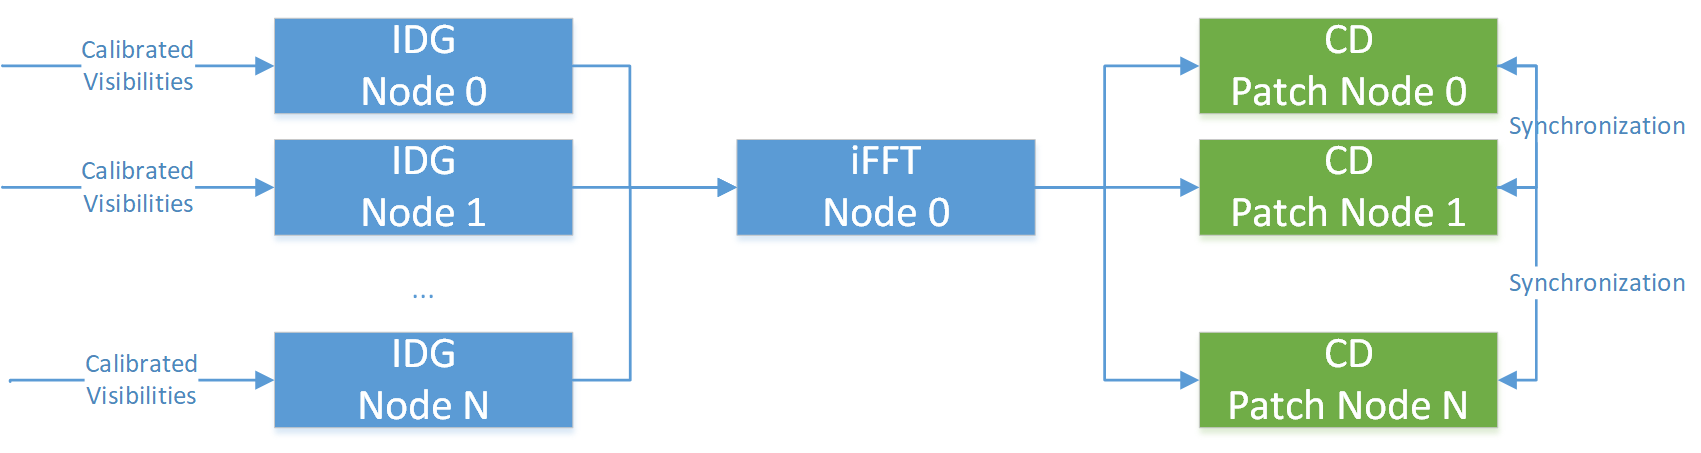
\includegraphics[width=0.80\linewidth]{./chapters/03.distribution/distributed_architecture.png}
	\caption{Distributed architecture for half a major cycle}
	\label{dist:architecture:fig}
\end{figure}

Where each node is one computer, i.e. has its own, possibly multiple cpus and its shared memory.
Split the input visibilities onto nodes. 
Do the gridding locally on each node
Communicate the grid
inverse FFT on one node.
Communicate the patches of the image.
Deconvolve each patch and communicate
